\documentclass{article}
\usepackage[utf8]{inputenc}
\usepackage[T1]{fontenc}
\usepackage[francais]{babel}
\usepackage{textcomp}
\usepackage{amsmath,amssymb,amsthm}
\usepackage{lmodern}
\usepackage[a4paper]{geometry}
\usepackage{graphicx}
\usepackage{xcolor}
\usepackage{multicol}
\usepackage{microtype}
\usepackage{pdfpages}
\usepackage{listings}
\usepackage{color}

\usepackage{hyperref}
\hypersetup{pdfstartview=XYZ}


\usepackage{fancyhdr}
\pagestyle{fancy}
\usepackage{lastpage}
\renewcommand\headrulewidth{0.4pt}
\fancyhead[L]{Casteleiro - Lefebvre - Vallet}
\fancyhead[R]{Prep'ISIMA}
\renewcommand\footrulewidth{0.4pt}
\fancyfoot[C]{
\textbf{Page \thepage/\pageref{LastPage}}}
\fancyfoot[R]{15/05/2020}

\definecolor{lightgray}{rgb}{0.92, 0.92, 0.92}

\lstset{frame=single,
backgroundcolor=\color{lightgray},
language=bash,
showstringspaces=false,
basicstyle={\small\ttfamily},
numbers=none,
tabsize=2,
}


\title{Rapport de projet : Lyapunov}
\date{}
\author{Projet réalisé par : Adrien Casteleiro, Antoine Lefebvre et Baptiste Vallet}
\AtEndDocument{\label{LastPage}}

\begin {document}
	\vspace*{-2pt}
	{\let\newpage\relax\maketitle} \thispagestyle{fancy}
	\begin{figure}[!h]
		\centering
		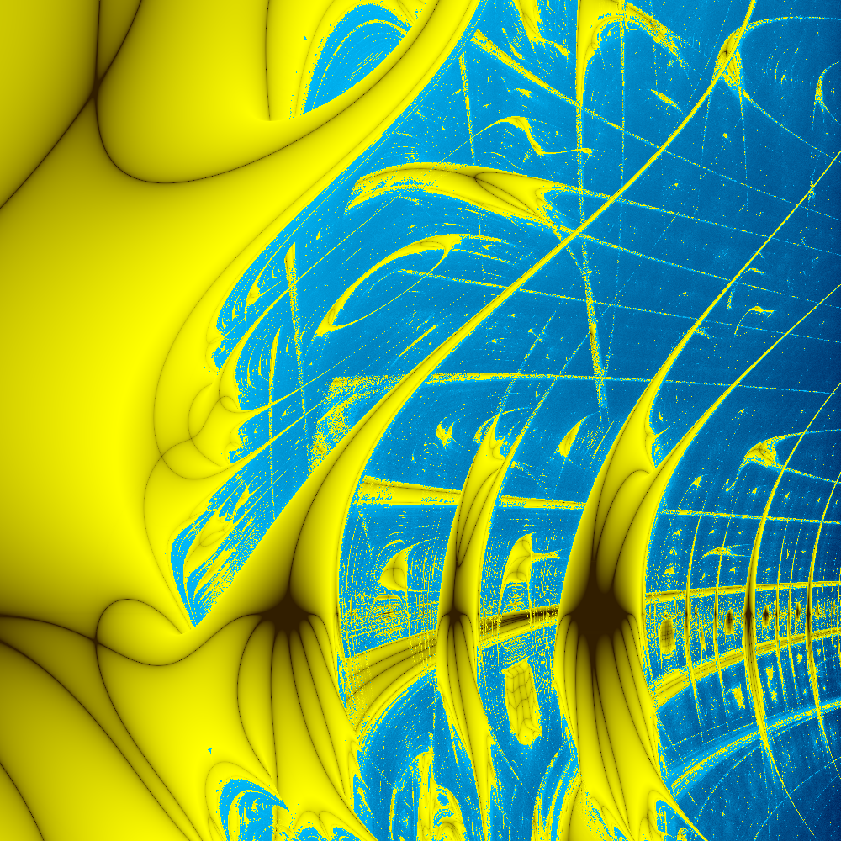
\includegraphics[scale=0.3]{zircon.png}
		\caption{Zircon City - Projet Lyapunov}
	\end{figure}
\newpage
	\tableofcontents
	\newpage
	\section{Installation}
	\subsection{Bibliothèques}
	\noindent Deux bibliothèques sont à installer:\\
	- Debian-based (Debian, Ubuntu, \ldots)
	\begin{lstlisting}
	$ sudo apt-get install libsdl2-dev
	\end{lstlisting}
	\begin{lstlisting}
	$ sudo apt-get install libgtkmm-3.0-dev
	\end{lstlisting}
	- RedHat-like (Fedora, CentOS, \ldots)
	\begin{lstlisting}
	$ sudo yum install libsdl2-dev
	\end{lstlisting}
	\begin{lstlisting}
	$ sudo yum install libgtkmm-3.0-dev
	\end{lstlisting}
	\subsection{Téléchargemement}
	\noindent Récupérer le dossier depuis le dépôt git:\\
	- SSH
	\begin{lstlisting}
	$ git clone git@gitlab.isima.fr:anlefebvre1/lyapunov.git
	\end{lstlisting}
	- HTTPS
	\begin{lstlisting}
	$ git clone https://gitlab.isima.fr/anlefebvre1/lyapunov.git
	\end{lstlisting}
	\subsection{Compiler - Exécuter}
	\noindent Se placer dans le dossier lyapunov
	\begin{lstlisting}
	$ cd lyapunov/
	\end{lstlisting}
	Exécuter la commande dans un terminal:
	\begin{lstlisting}
	$ make
	\end{lstlisting}
	Exécuter ensuite la commande pour lancer l'exécutable:
	\begin{lstlisting}
	$ ./lyapunov
	\end{lstlisting}

	\section{Présentation du programme}
	\subsection{Menu}
	En lançant le programme, un menu est affiché afin de choisir les couleurs représentants les valeurs des exposants de Lyapunov, la précision voulue, c'est à dire le nombre d'itérations pour calculer un exposant, et la séquence qui sera utilisée.
	En appuyant sur Valider, la génération est lancée et les fractales s'affichent.
	Si l'utilisateur ne rentre pas de séquence lors de la première ouverture du menu, alors une séquence est générée aléatoirement afin de permettre à l'utilisateur de découvrir de nouvelles fractales.
	L'utilisateur peut récupérer la séquence aléatoire via la console.
	Le menu peut être ré-ouvert en utilisant la touche Echap pour modifier les couleurs, ou changer la précision / séquence.
	Si la séquence est laissée vide lors de la réouverture du menu, alors la dernière séquence sera prise en compte sans que l'utilisateur n'ait à entrer une nouvelle fois la séquence.

	\subsection{Navigation}
	La navigation se fait avec les flèches directionnelles (haut, bas, gauche, droit), permettant de se déplacer d'un demi-écran.
	Le zoom se fait avec le clic gauche de la souris, et la zone où l'on va zoomer est représenté par un carré blanc autour du pointeur de la souris.
	Le dézoom s'effectue avec le clic droit, pour revenir à la zone avant le zoom.
	Pour modifier la puissance du zoom, on utilise la molette de la souris.
	\subsection{Exportation}
	Pour exporter ce qui apparait à l'écran, on utilise la touche Entrée.
	La capture d'écran se trouvera dans le dossier 'screenshot' au format bmp.
	\section{Fonctionnement}
	\subsection{Gérer la SDL}
	Pour afficher la fractale, il a fallu travailler avec la SDL, qui est une bibliothèque écrite en C, et donc l'adapter en C++ avec un wrapper, qui est la classe Window Manager.
	Le but de cette classe est ainsi de pouvoir travailler avec la SDL en évitant les pointeurs, et permettre un découplage entre la SDL et notre programme.
	Cette classe utilise une texture pour modifier les pixels que l'on veut afficher, et un render (qui est un élément de la SDL) pour afficher la texture à l'écran.
	On peut ainsi afficher la fractale facilement sans avoir à se préoccuper du fonctionnement au niveau de la SDL.
	Le programme fonctionne avec une boucle d'évènement, et pour chaque évènement qui nous intéresse, on peut le traiter avec une fonction évènementielle en dehors de la classe s'occupant de la SDL.

	\subsection{Génération et affichage}
	Les fractales de Lyapunov sont une certaine représentation d'une suite chaotique calculée à partir des exposants de Lyapunov.
	L'algorithme de génération des fractales de Lyapunov en 2D dans le plan $[0,4] \times [0,4]$ est séparée en plusieurs étapes.
	Tout d'abord, on choisit une séquence de A et B.
	On construit ensuite une séquence $S_n$ suffisament longue constituée d'une répétiton de la séquence de A et B définie précedemment.
	On choisit un point de coordonées x,y dans le plan de depart.
	On définit ensuite la fonction $R_n = a$ si $ S_n = A $ et $R_n = b$ sinon.
	On construit ensuite une suite $x_n$ notée $x_{{n+1}}=r_{n}x_{n}(1-x_{n})$ en prenant comme origine $x_0 = 0.5$.
	On calcule ensuite l'exposant de Lyapunov noté $\lambda$ grâce à cette formule:
	\[
		\lambda = \lim_{N \to +\infty} \frac{1}{N} \sum_{n=1}^{N} \log | r_n(1-2x_n) |
	\]
	Ensuite, pour afficher les fractales à l'écran, on attribue une couleur à chaque exposant afin de pouvoir changer les couleurs à la volée, qui sont représentées en RGB.
	Nous avons essayé beaucoup de représentations différentes, ainsi qu'une représentation arc-en-ciel en mouvement.

	\subsection{Optimisation et multi-threading}

	L'opération la plus coûteuse dans le calcul de l'exposant est le logarithme, mais puisqu'on réalise des sommes de logarithmes, on peut alors utiliser la propriété $\log(a) + \log(b) = \log(a \times b)$.
	Lorsqu'on atteint une certaine limite (ici $1.10^{100}$: le type double nous permet d'atteindre ces valeurs suffisament élevées), on prend le logarithme du produit que l'on ajoute au résultat final.
	Ainsi, il y a moins de logarithmes à calculer et on gagne en temps de calcul.
	Afin d'améliorer la vitesse de calcul et d'affichage des fractales de Lyapunov, on utilise aussi la parallélisation.
	On récupère le nombre de threads du processeur et on découpe ensuite la génération à partir d'un bloc en plusieurs blocs correspondant à chacun une région de la fractale.
	Nous avons décidé de séparer les différentes régions de la fractale à partir du nombre de "lignes" dans notre tableau.
	Pour cela, on utilise la bibliothèque <thread> native, qui est assez simple d'utilisation dans notre cas.
	En effet, en séparant les calculs des exposants sur différents threads, il est possible de gagner un temps assez conséquent lors du calcul de la fractale.

	\subsection{Les couleurs}

	Les couleurs sont obtenues depuis le fichier de configuration.
	Ensuite, on stocke dans un tableau et répartis selon les composantes rouges, vertes, et bleues, les différences entre la couleur maximale et minimale suivant le signe de l'exposant, puis la couleur à qui cette différence a été imputée.
	Les valeurs maximale et minimale de l'exposant de la région calculée sont stockées, pour créer une échelle de couleurs suivant le signe.
	Pour chaque composante de couleur, la différence de couleur est multipliée par la division de l'exposant par la borne adaptée et enfin ajoutée à la couleur stockée.

	\subsection{Interactions avec l'utilisateur}

	Afin de pouvoir interagir avec la fractale, on a besoin de pouvoir convertir les coordonnées écrans en coordonnées de Lyapunov.
	Avec cela, on utilise une région, qui définit les coordonnées de départ et d'arrivée sur les deux axe.
	Pour convertir, on divise, pour chaque coordonnées, la différence entre le nouveau et l'ancien point par la largeur de la texture, puis on multiplie par la largeur actuelle et on ajoute l'origine.

	\subsubsection{Le zoom}

	En zoomant, on récupère la région en convertissant les coordonnées écrans, et on calcule la zone à afficher avec cette région.
	Pour pouvoir dézoomer, on conserve chaque région avant de zoomer que l'on place dans une pile.
	À chaque clic droit, on récupère cette région et on recalcule pour ré-afficher l'ancienne fractale

	\subsubsection{Le déplacement}

	La zone où l'on veut se déplacer est calculée selon la région actuelle en ajoutant le demi-écran.
	Si on essaye de se déplacer en dehors de la bordure, la région reste collée à la bordure.


	\subsection{Le menu}
	Le menu a été réalisé avec la bibliothèque <GTKmm>, la version en C++ de GTK+, la bibliothèque graphique de GIMP notamment.
	Elle dispose de nombreuses classes afin de permettre à l'utilisateur de créer des interfaces graphiques et des menus de navigation très facilement.
	Nous avons donc opté pour cette libraire afin d'implémenter le menu car elle dispose de nombreux widgets comme des selecteurs de couleurs, ou bien encore des zones de saisie de texte afin de permettre à l'utilisateur de pouvoir choisir la séquence et les couleurs entre autres .
	Le menu fait principalement appel à plusieurs petites fonctions qui lui permettent de compléter plus facilement le fichier de configuration.
	Nous avons décidé d'écrire les différents choix de l'utilisateur dans un ficher de configuration afin de pouvoir récuperer facilement et rapidement les valeurs entre les différentes classes sans avoir à passer par un accesseur par exemple.
	Le menu est capable d'écrire les différentes couleurs sous la forme 255 255 255, la séquence saisie et aussi la précision souhaitée par l'utilisateur dans le fichier de configuration.

	\section{Les choix}

	\subsection{Le langage}
	Nous avons décidé d'utiliser le langage C++ car c'est un langage nouveau pour nous, et il est intéressant de le maîtriser.

	\subsection{La bibliothèque graphique}
	Nous avons utilisé la SDL car c'est une bibliothèque que nous connaissons, et bien qu'elle fut créée pour le C, il est possible de l'utiliser pour le C++.
	Nous avons étudié d'autres libraries mais elles semblaient moins adapté pour de l'affichage pixel par pixel.
	Nous avons également utilisé GTKmm pour la création d'un menu grâce à sa facilité d'utilisation et de création d'interfaces graphiques.

	\section{Les difficultés rencontrées}

	\subsection{Le menu}
	Le menu a été une source de quelques difficultés.
	Nous avons décidé de nous orienter vers GTKmm, la version de GTK+ pour le C++.
	GTKmm dispose de nombreux widgets, comme des boutons ou des saisies de texte afin de permettre la création de menu plus facilement qu'en SDL, où l'on doit tout créer.
	La première et principale difficulté que nous avons rencontrée lors de la création du menu était d'apprendre le fonctionnement des bibliothèques de GTK. Il a fallu apprendre l'utilisation et les normes de GTKmm qui sont très différentes de la SDL que nous connaissions déjà.
	La création du menu n'a requis que les bases de GTKmm réduisant ainsi la durée d'apprentissage.
	Le menu a également posé des problèmes de mise en forme.
	En effet, la première version du menu utilisait des box afin de contenir les différents widgets de GTK comme les boutons ou les labels.
	Mais, il n'etait pas possible de placer précisement les éléments à l'intérieur du conteneur.
	On a alors décidé de s'orienter vers une "grid", un conteneur qui permet lui de séparer la fenêtre du menu en plusieurs compartiments.
	Il était alors beaucoup plus facile de pouvoir positionner les différents éléments qui composent le menu.
	Mais, un autre problème était source de difficultés : l'affichage des textes à côté des boutons.
	GTKmm dispose de "labels" qui sont censés permettre à l'utilisateur d'écrire du texte.
	Mais, il suffisait juste de remplacer les "labels" par une de ses sous classes "AccelLabel".

	\subsection{Le multi-threading}
	La difficulté principale du multi-threading / parallélisation était de comprendre les différents concepts du multi-threading.
	Une fois, les notions comprises, l'implémentation a été réalisée dans la foulée sans grande difficulté supplémentaire en "découpant" la génération en plusieurs parties.

	\subsection{Effets d'image}

	Originellement, nous avions prévu d'octroyer à l'utilisateur la possibilité de tourner la texture de 90° ou de la renverser à volonté.
	Cependant, notre manière de récupérer la région cliquée n'était pas compatible avec le fait de pouvoir faire des rotations.
	Une tentative a néanmoins été faite, nous permettant de faire une rotation et de zoomer correctement, mais cela ne marchait que pour le premier niveau de zoom.
	Nous avons jugé que cette fonctionnalité n'était pas très importante, et que changer notre implémantation n'en aurait pas valu la peine, puisque la rotation peut se faire facilement par l'utilisateur à l'aide d'un éditeur d'image après exportation.

	\section{Répartition des tâches}

	\subsection*{Adrien}
	\begin{itemize}
		\item Première version du projet : PPM.
		\item Première version du traitement des couleurs avec Antoine.
		\item Première version de l'optimisation du calcul des exposants de Lyapunov.
		\item Création + Fonctionnement du menu en interaction avec l'utilisateur.
		\item Choix des couleurs + Séquence + Précision.
		\item Vérification + Traitement de la séquence : séquence aléatoire en fonction de la précision.
		\item Traitement des données du fichier de configuration.
		\item Paralléliation - Multi-threading.
	\end{itemize}

	\subsection*{Antoine}

	\begin{itemize}
		\item Création du wrapper de la SDL (WindowManager)
		\item Boucle d'évènement + fonctions évènementielles
		\item Capture d'écran
		\item Zoom + afficher la zone où l'on va zoomer + régler la puissance du zoom
		\item Dézoom
		\item Conversion des coordonnées écran en coordonnées Lyapunov
		\item Test de la couleur arc-en-ciel bougeante (fonction HSV)
		\item Classes Region + Time
		\item Version finale de l'optimisation de calcul
		\item Tentative de l'orientation
	\end{itemize}

	\subsection*{Baptiste}
	
	\begin{itemize}
		\item Recherche d'effets SDL sur texture
		\item Implémentation d'effets de rotation et de renversements de l'image (supprimés du code final)
		\item Algorithme d'attribution des couleurs en dégradé
		\item Déplacement
	\end{itemize}


\end {document}
